\section{Door task}
	\label{sub:door}

\subsection{Outline}
%
The door task consists of the following four sequential steps.
%
\begin{description}
\item{Step1} Locate a door in the environment
\item{Step2} Walk to the front of the door and grasp the door knob
\item{Step3} Turn the knob and open the door
\item{Step4} Walk through the door
\end{description}
%

%In the DRC Finals, it was announced that the door will be 
%
%\begin{itemize}
%\item push open style,
%\item with lever type door knob, and
%\item without door closer.
%\end{itemize}

To realize a reliable door passing, we pre-determined
a robot pose grasping the door knob.
Let us call it as {\it door approaching pose} which specifies the
wrist point and the standing point with respect to the door lever
as illustrated in \figurename~\ref{fig:door_approaching_config}.

From Step1 to Step2, we control our robot to realize the door approaching pose.
The door knob operation (Step3) and the door passing through (Step4) always start
from this fixed configuration. This means we can use a programmed sequence or its minimum
modification at the door task.  

\begin{figure}[t]
  \centering
  \includegraphics[width = 6cm]{img/door_approaching_config}
  \caption{Door approaching pose}
  \label{fig:door_approaching_config}
\end{figure}
        
\subsection{Detection of the door lever}
%
For a door task, a robot must detect the door orientaion and the position 
of the door lever. We took two step manual operations to extract the required information
from the point cloud. % as illustrated in Fig.\ref{fig:door_manip_markers}.

First, an operator specifies an ``attention point'' on the point cloud which might correspond the 
left edge of the door panel (\figurename~\ref{fig:door_manip_markers}(a)). We can expect a flat plane 
on the right of the attention point, and we can calculate the orientation of the door plane by the least square method.
In \figurename~\ref{fig:door_manip_markers}(b) shows the automatically alligned ``door manipulation marker.''
The marker covers a part of the door panel and we can interactively manipulate it on the 
pointcloud GUI. By manually translating the marker, we can mask the flat portion of 
the point cloud and extract the door lever as shown in \figurename~\ref{fig:door_manip_markers}(c).
Since the door lever is relatively small with respect to the point cloud resolution,
it contains only 10 to 20 points which makes conventional model fitting very difficult.
Thanks to the robustness of the human perception, we can confidently assume the rotation center of the lever
 and the model allignment on the point cloud as \figurename~\ref{fig:door_manip_markers}(d).

\begin{figure}[t]
  \centering
  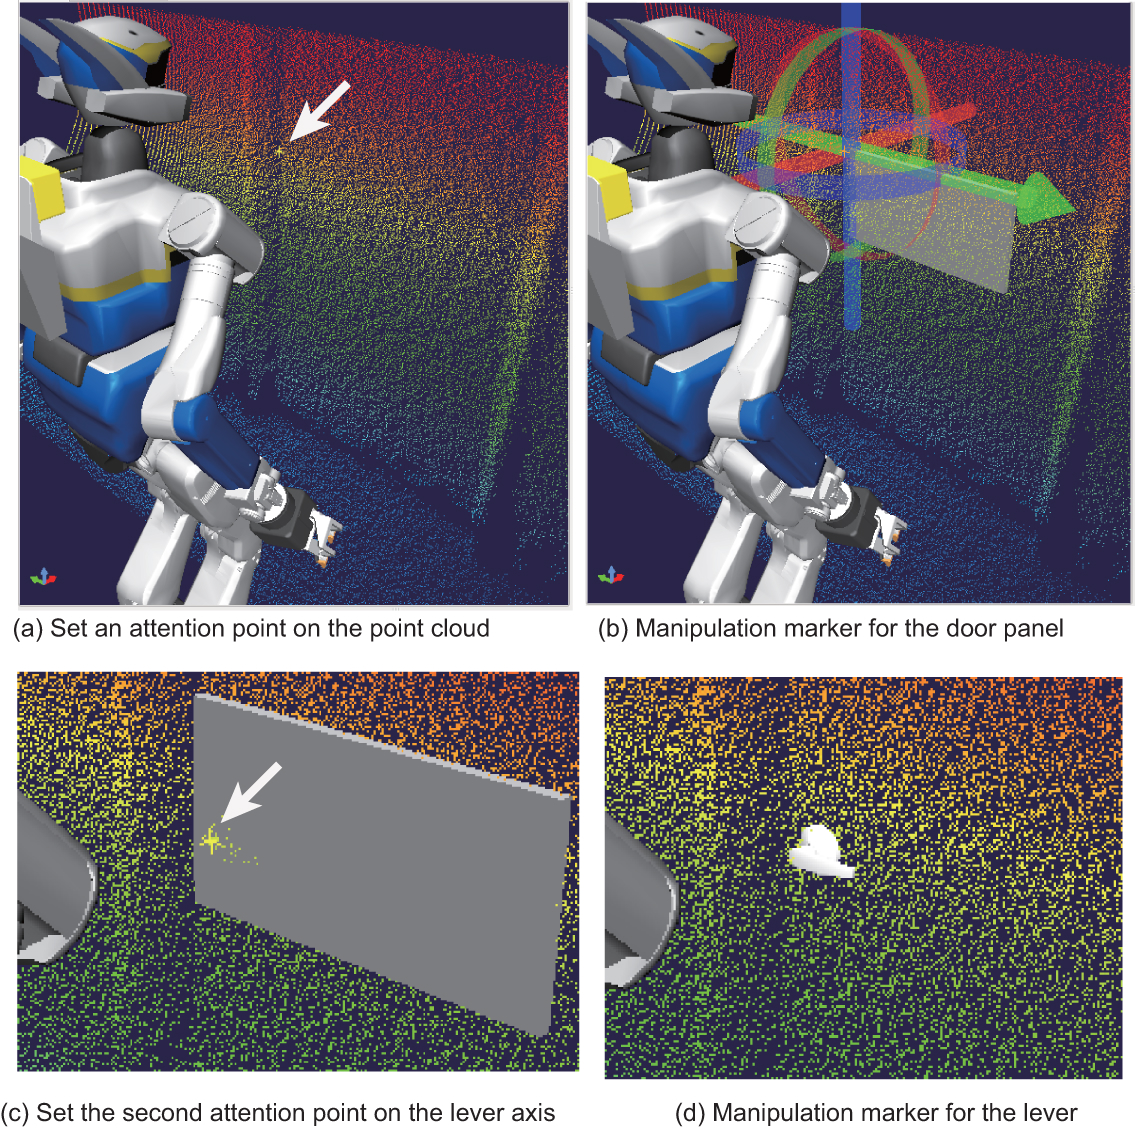
\includegraphics[width = 7.5cm]{img/door_manipulation_markers}
  \caption{Detection of the door lever in the control window}
  \label{fig:door_manip_markers}
\end{figure}
		

\subsection{Door lever grasp and manipulation}
%
By the method of previous subsection, we can expect 
our robot is standing in front of the door aligned to its surface normal with desired
distance. 
Nevertheless, due to the LRF measurement noise and its callibration error,
the hand position may not be acculate enough to grasp the lever. Such state in the dynamic simulation 
of Choreonoid is shown in \figurename~\ref{fig:door_lever_grasp}(a). 
The right window shows the simulated robot and the left 
window shows the view of the left hand camera. An operator can fix this manually by the GUI buttons of 
'Left','Right','Down', and 'Up' as seen in the left window bottom. In this case, an operator
can adjust the hand position by clicking 'Right' button several times.
Figure \ref{fig:door_lever_grasp}(b) shows the adjusted hand position to grasp the lever.
By hitting the button `OK', the robot move the left hand forward until it contacts the door surface (we specified a sleshold of 5N to detect the contact).  The hand is in contact with appropriate position to grasp the door lever in \figurename~\ref{fig:door_lever_grasp}(c).
   

\begin{figure}[t]
  \centering
  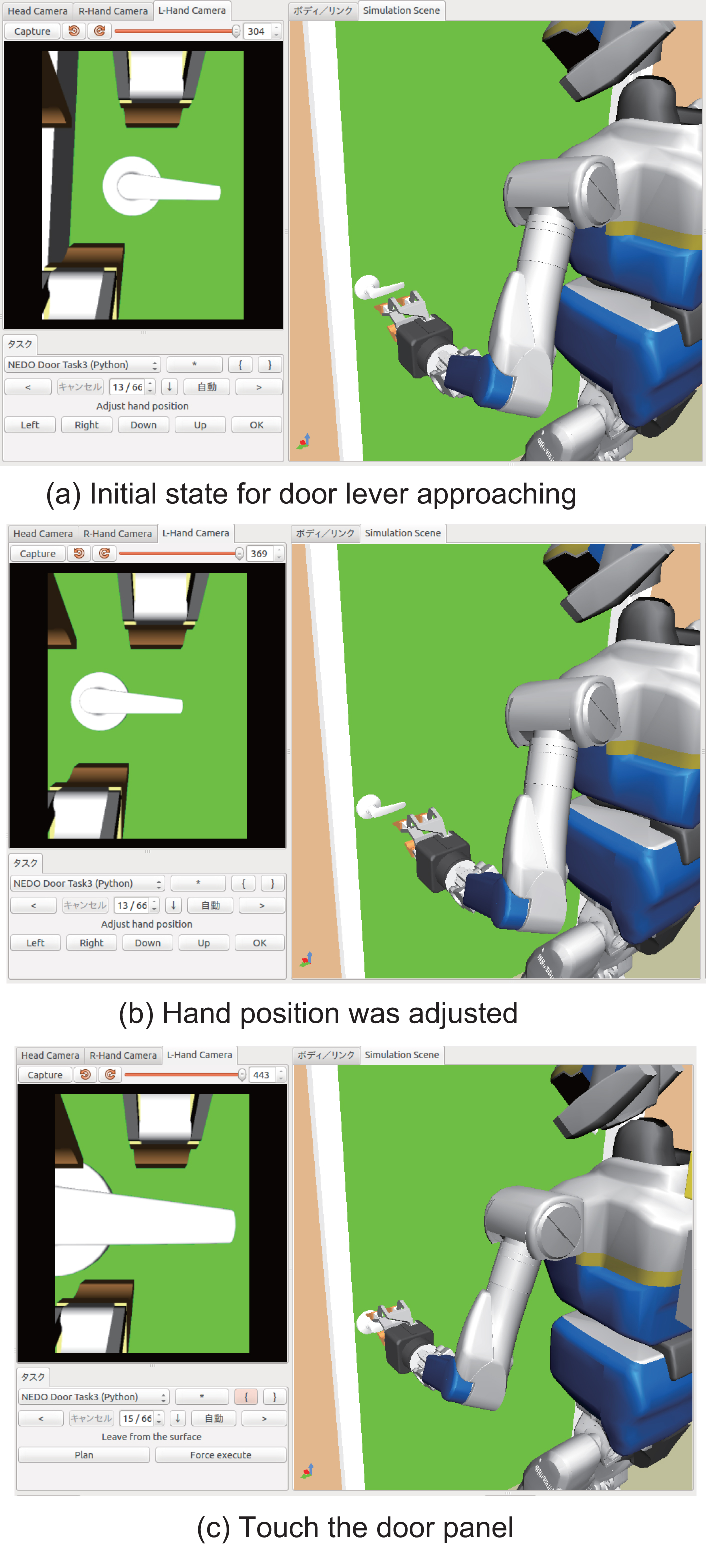
\includegraphics[width = 7.5cm]{img/approach_door_lever}
  \caption{Approach for door lever grasping}
  \label{fig:door_lever_grasp}
\end{figure}

%\begin{figure}[t]
%  \centering
%  \includegraphics[width = 7.5cm]{img/open_the_door.eps}
%  \caption{Door opening}
%  \label{fig:door_opening}
%\end{figure}

\subsection{Results at DRC Finals}
%
In the DRC Finals, the task stage floor has a slope of 2.6 degrees by 
our measurement, and the door was set perpendicular to the slope. 
By this setup, once the door was enough opend it quickly open by gravity
and remained opening state. This helped a lot our robot to pass the door.

On the other hand, we found that the door of each course has a different latch property
as shown in Table.\ref{tbl:door_latch}.

%
\begin{table}[htb]
\caption{Door latch properties at DRC finals} \label{tbl:door_latch}
\begin{tabular}{lclc}
\hline
Course & Lever angle to open & Date & Result  \\ 
\hline
Green & 30 deg & June 4 (rehasal) & Success  \\
Yellow & 70 deg & June 5 (day1) & Fail \\
Blue &  50 deg & June 6 (day2)  & Success \\
\hline
\end{tabular}
\end{table}

our robot had a trouble on turning the lever and releasing the latch.